\documentclass[a4paper]{book}
\usepackage{makeidx}
\usepackage{natbib}
\usepackage{graphicx}
\usepackage{multicol}
\usepackage{float}
\usepackage{listings}
\usepackage{color}
\usepackage{ifthen}
\usepackage[table]{xcolor}
\usepackage{textcomp}
\usepackage{alltt}
\usepackage{ifpdf}
\ifpdf
\usepackage[pdftex,
            pagebackref=true,
            colorlinks=true,
            linkcolor=blue,
            unicode
           ]{hyperref}
\else
\usepackage[ps2pdf,
            pagebackref=true,
            colorlinks=true,
            linkcolor=blue,
            unicode
           ]{hyperref}
\usepackage{pspicture}
\fi
\usepackage[utf8]{inputenc}
\usepackage[ngerman]{babel}

\usepackage{mathptmx}
\usepackage[scaled=.90]{helvet}
\usepackage{courier}
\usepackage{sectsty}
\usepackage[titles]{tocloft}
\usepackage{doxygen}
\lstset{language=C++,inputencoding=utf8,basicstyle=\footnotesize,breaklines=true,breakatwhitespace=true,tabsize=8,numbers=left }
\makeindex
\setcounter{tocdepth}{3}
\renewcommand{\footrulewidth}{0.4pt}
\renewcommand{\familydefault}{\sfdefault}
\hfuzz=15pt
\setlength{\emergencystretch}{15pt}
\hbadness=750
\tolerance=750
\begin{document}
\hypersetup{pageanchor=false,citecolor=blue}
\begin{titlepage}
\vspace*{7cm}
\begin{center}
{\Large \-P\-T100 \-Library }\\
\vspace*{1cm}
{\large \-Erzeugt von Doxygen 1.7.6.1}\\
\vspace*{0.5cm}
{\small Mit Jul 18 2012 11:43:43}\\
\end{center}
\end{titlepage}
\clearemptydoublepage
\pagenumbering{roman}
\tableofcontents
\clearemptydoublepage
\pagenumbering{arabic}
\hypersetup{pageanchor=true,citecolor=blue}
\chapter{\-Datei-\/\-Verzeichnis}
\section{\-Auflistung der \-Dateien}
\-Hier folgt die \-Aufzählung aller \-Dateien mit einer \-Kurzbeschreibung\-:\begin{DoxyCompactList}
\item\contentsline{section}{\hyperlink{pt100__table_8h}{pt100\-\_\-table.\-h} \\*\-Tabelle mit \-P\-T100-\/\-Widerstandswerten von \mbox{[}-\/200 ... +850\mbox{]}°\-C in 1\-K-\/\-Schritten }{\pageref{pt100__table_8h}}{}
\item\contentsline{section}{\hyperlink{pt100__types_8h}{pt100\-\_\-types.\-h} \\*\-Typdefinitionen der \-P\-T100-\/\-Lib }{\pageref{pt100__types_8h}}{}
\item\contentsline{section}{\hyperlink{pt100lib_8c}{pt100lib.\-c} \\*\-Bibiliothek mit \-P\-T100 \-Funktionen }{\pageref{pt100lib_8c}}{}
\item\contentsline{section}{\hyperlink{pt100lib_8h}{pt100lib.\-h} \\*\-Bibiliothek mit \-P\-T100 \-Funktionen }{\pageref{pt100lib_8h}}{}
\end{DoxyCompactList}

\chapter{\-Datei-\/\-Dokumentation}
\hypertarget{pt100__table_8h}{
\section{/home/rb/workspace/pt100lib/private/pt100\_\-table.h-\/Dateireferenz}
\label{pt100__table_8h}\index{/home/rb/workspace/pt100lib/private/pt100\_\-table.h@{/home/rb/workspace/pt100lib/private/pt100\_\-table.h}}
}


Tabelle mit PT100-\/Widerstandswerten von \mbox{[}-\/200 ... +850\mbox{]}°C in 1K-\/Schritten.  


\subsection*{Makrodefinitionen}
\begin{DoxyCompactItemize}
\item 
\#define \hyperlink{pt100__table_8h_a58cacf232e018f6c32af1f496a7a9aa0}{R\_\-MIN}~18493L
\begin{DoxyCompactList}\small\item\em Minimaler Widerstandswert in mOhm. \item\end{DoxyCompactList}\item 
\#define \hyperlink{pt100__table_8h_a44d864c7ff8bf7f56435a1226c9e8a99}{R\_\-MAX}~390263L
\begin{DoxyCompactList}\small\item\em Maximaler Widerstandswert in mOhm. \item\end{DoxyCompactList}\item 
\#define \hyperlink{pt100__table_8h_a0e37b765046be143ca51ec097adf606a}{T\_\-MIN}~-\/200000L
\begin{DoxyCompactList}\small\item\em Minimale Temperatur der Widerstandstabelle in m°C. \item\end{DoxyCompactList}\item 
\#define \hyperlink{pt100__table_8h_acd0dda75fa865e1efae98e3e2b204ef4}{T\_\-MAX}~850000L
\begin{DoxyCompactList}\small\item\em Maximale Temperatur der Widerstandstabelle in m°C. \item\end{DoxyCompactList}\item 
\#define \hyperlink{pt100__table_8h_a993bb708226c81076621cb7eb014eaba}{T\_\-DIFF}~1000L
\begin{DoxyCompactList}\small\item\em Temperaturintervall der Widerstandstabelle in mK. \item\end{DoxyCompactList}\item 
\#define \hyperlink{pt100__table_8h_a26db5af8ea96c4eb44a373ca5c41f494}{INDEX\_\-MAX}~1050
\begin{DoxyCompactList}\small\item\em Maximaler Index der PT100-\/Tabelle. \item\end{DoxyCompactList}\item 
\#define \hyperlink{pt100__table_8h_ad65514e056b8be6706716483611e9463}{INDEX\_\-ZERO}~200
\begin{DoxyCompactList}\small\item\em Index für 0°C in der PT100-\/Tabelle. \item\end{DoxyCompactList}\end{DoxyCompactItemize}
\subsection*{Variablen}
\begin{DoxyCompactItemize}
\item 
unsigned long const \hyperlink{pt100__table_8h_afbf775603ef1f6f0ef7d4a0af6a490c0}{pt100\_\-table} \mbox{[}$\,$\mbox{]}
\begin{DoxyCompactList}\small\item\em Tabelle mit PT100-\/Widerstandswerten von \mbox{[}-\/200 ... +850\mbox{]}°C in 1K-\/Schritten. \item\end{DoxyCompactList}\end{DoxyCompactItemize}


\subsection{Ausführliche Beschreibung}
Tabelle mit PT100-\/Widerstandswerten von \mbox{[}-\/200 ... +850\mbox{]}°C in 1K-\/Schritten. \begin{DoxyAuthor}{Autor}
Roman Buchert (\href{mailto:roman.buchert@googlemail.com}{\tt roman.buchert@googlemail.com}) 
\end{DoxyAuthor}


Definiert in Datei \hyperlink{pt100__table_8h_source}{pt100\_\-table.h}.



\subsection{Makro-\/Dokumentation}
\hypertarget{pt100__table_8h_a26db5af8ea96c4eb44a373ca5c41f494}{
\index{pt100\_\-table.h@{pt100\_\-table.h}!INDEX\_\-MAX@{INDEX\_\-MAX}}
\index{INDEX\_\-MAX@{INDEX\_\-MAX}!pt100_table.h@{pt100\_\-table.h}}
\subsubsection[{INDEX\_\-MAX}]{\setlength{\rightskip}{0pt plus 5cm}\#define INDEX\_\-MAX~1050}}
\label{pt100__table_8h_a26db5af8ea96c4eb44a373ca5c41f494}


Maximaler Index der PT100-\/Tabelle. 



Definiert in Zeile 37 der Datei pt100\_\-table.h.



Wird benutzt von pt100\_\-R2T() und pt100\_\-T2R().

\hypertarget{pt100__table_8h_ad65514e056b8be6706716483611e9463}{
\index{pt100\_\-table.h@{pt100\_\-table.h}!INDEX\_\-ZERO@{INDEX\_\-ZERO}}
\index{INDEX\_\-ZERO@{INDEX\_\-ZERO}!pt100_table.h@{pt100\_\-table.h}}
\subsubsection[{INDEX\_\-ZERO}]{\setlength{\rightskip}{0pt plus 5cm}\#define INDEX\_\-ZERO~200}}
\label{pt100__table_8h_ad65514e056b8be6706716483611e9463}


Index für 0°C in der PT100-\/Tabelle. 



Definiert in Zeile 41 der Datei pt100\_\-table.h.



Wird benutzt von pt100\_\-R2T().

\hypertarget{pt100__table_8h_a44d864c7ff8bf7f56435a1226c9e8a99}{
\index{pt100\_\-table.h@{pt100\_\-table.h}!R\_\-MAX@{R\_\-MAX}}
\index{R\_\-MAX@{R\_\-MAX}!pt100_table.h@{pt100\_\-table.h}}
\subsubsection[{R\_\-MAX}]{\setlength{\rightskip}{0pt plus 5cm}\#define R\_\-MAX~390263L}}
\label{pt100__table_8h_a44d864c7ff8bf7f56435a1226c9e8a99}


Maximaler Widerstandswert in mOhm. 



Definiert in Zeile 21 der Datei pt100\_\-table.h.



Wird benutzt von pt100\_\-R2T().

\hypertarget{pt100__table_8h_a58cacf232e018f6c32af1f496a7a9aa0}{
\index{pt100\_\-table.h@{pt100\_\-table.h}!R\_\-MIN@{R\_\-MIN}}
\index{R\_\-MIN@{R\_\-MIN}!pt100_table.h@{pt100\_\-table.h}}
\subsubsection[{R\_\-MIN}]{\setlength{\rightskip}{0pt plus 5cm}\#define R\_\-MIN~18493L}}
\label{pt100__table_8h_a58cacf232e018f6c32af1f496a7a9aa0}


Minimaler Widerstandswert in mOhm. 



Definiert in Zeile 17 der Datei pt100\_\-table.h.



Wird benutzt von pt100\_\-R2T().

\hypertarget{pt100__table_8h_a993bb708226c81076621cb7eb014eaba}{
\index{pt100\_\-table.h@{pt100\_\-table.h}!T\_\-DIFF@{T\_\-DIFF}}
\index{T\_\-DIFF@{T\_\-DIFF}!pt100_table.h@{pt100\_\-table.h}}
\subsubsection[{T\_\-DIFF}]{\setlength{\rightskip}{0pt plus 5cm}\#define T\_\-DIFF~1000L}}
\label{pt100__table_8h_a993bb708226c81076621cb7eb014eaba}


Temperaturintervall der Widerstandstabelle in mK. 



Definiert in Zeile 33 der Datei pt100\_\-table.h.



Wird benutzt von pt100\_\-R2T() und pt100\_\-T2R().

\hypertarget{pt100__table_8h_acd0dda75fa865e1efae98e3e2b204ef4}{
\index{pt100\_\-table.h@{pt100\_\-table.h}!T\_\-MAX@{T\_\-MAX}}
\index{T\_\-MAX@{T\_\-MAX}!pt100_table.h@{pt100\_\-table.h}}
\subsubsection[{T\_\-MAX}]{\setlength{\rightskip}{0pt plus 5cm}\#define T\_\-MAX~850000L}}
\label{pt100__table_8h_acd0dda75fa865e1efae98e3e2b204ef4}


Maximale Temperatur der Widerstandstabelle in m°C. 



Definiert in Zeile 29 der Datei pt100\_\-table.h.



Wird benutzt von pt100\_\-T2R().

\hypertarget{pt100__table_8h_a0e37b765046be143ca51ec097adf606a}{
\index{pt100\_\-table.h@{pt100\_\-table.h}!T\_\-MIN@{T\_\-MIN}}
\index{T\_\-MIN@{T\_\-MIN}!pt100_table.h@{pt100\_\-table.h}}
\subsubsection[{T\_\-MIN}]{\setlength{\rightskip}{0pt plus 5cm}\#define T\_\-MIN~-\/200000L}}
\label{pt100__table_8h_a0e37b765046be143ca51ec097adf606a}


Minimale Temperatur der Widerstandstabelle in m°C. 



Definiert in Zeile 25 der Datei pt100\_\-table.h.



Wird benutzt von pt100\_\-T2R().



\subsection{Variablen-\/Dokumentation}
\hypertarget{pt100__table_8h_afbf775603ef1f6f0ef7d4a0af6a490c0}{
\index{pt100\_\-table.h@{pt100\_\-table.h}!pt100\_\-table@{pt100\_\-table}}
\index{pt100\_\-table@{pt100\_\-table}!pt100_table.h@{pt100\_\-table.h}}
\subsubsection[{pt100\_\-table}]{\setlength{\rightskip}{0pt plus 5cm}unsigned long const {\bf pt100\_\-table}\mbox{[}$\,$\mbox{]}}}
\label{pt100__table_8h_afbf775603ef1f6f0ef7d4a0af6a490c0}


Tabelle mit PT100-\/Widerstandswerten von \mbox{[}-\/200 ... +850\mbox{]}°C in 1K-\/Schritten. 

Die Werte sind in mOhm angegeben 

Definiert in Zeile 51 der Datei pt100\_\-table.h.



Wird benutzt von pt100\_\-R2T() und pt100\_\-T2R().


\hypertarget{pt100__types_8h}{
\section{/home/rb/workspace/pt100lib/includes/pt100\_\-types.h-\/Dateireferenz}
\label{pt100__types_8h}\index{/home/rb/workspace/pt100lib/includes/pt100\_\-types.h@{/home/rb/workspace/pt100lib/includes/pt100\_\-types.h}}
}


Typdefinitionen der PT100-\/Lib.  


Dieser Graph zeigt, welche Datei direkt oder indirekt diese Datei enthält:
\nopagebreak
\begin{figure}[H]
\begin{center}
\leavevmode
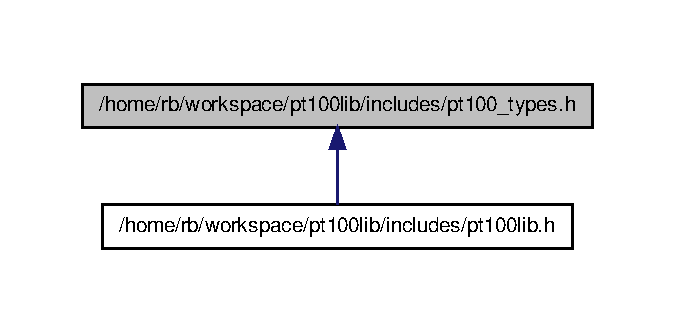
\includegraphics[width=324pt]{pt100__types_8h__dep__incl}
\end{center}
\end{figure}
\subsection*{Typdefinitionen}
\begin{Indent}{\bf Typdefinitionen unsigned}\par
\begin{DoxyCompactItemize}
\item 
typedef unsigned char \hyperlink{pt100__types_8h_ab291f552d5fd4d65ac668d6b2b180919}{\_\-\_\-u8}
\item 
typedef unsigned short \hyperlink{pt100__types_8h_ac915988d8c60a3b943f936c25f9eca6e}{\_\-\_\-u16}
\item 
typedef unsigned long \hyperlink{pt100__types_8h_a13a2835755bfba96b1790ff492741141}{\_\-\_\-u32}
\item 
typedef unsigned long long \hyperlink{pt100__types_8h_a0d73388ab5d53ebb5368677f33ff9c63}{\_\-\_\-u64}
\end{DoxyCompactItemize}
\end{Indent}
\begin{Indent}{\bf Typdefinitionen unsigned, nur lesend}\par
\begin{DoxyCompactItemize}
\item 
typedef unsigned char const \hyperlink{pt100__types_8h_afbecaec6b78809bfcb9a77e44e1d1f6d}{\_\-\_\-uc8}
\item 
typedef unsigned short const \hyperlink{pt100__types_8h_ac3fe55ac77a001b6e6ce9a56d2898c4d}{\_\-\_\-uc16}
\item 
typedef unsigned long const \hyperlink{pt100__types_8h_a8fbd842df23a12cc032e5c0b2f0f1b2b}{\_\-\_\-uc32}
\item 
typedef unsigned long long const \hyperlink{pt100__types_8h_a736c156c3f292472efee5a420c1553fa}{\_\-\_\-uc64}
\end{DoxyCompactItemize}
\end{Indent}
\begin{Indent}{\bf Typdefinitionen signed}\par
\begin{DoxyCompactItemize}
\item 
typedef signed char \hyperlink{pt100__types_8h_a9e371a4230da8dd05ce434b233a5f8d0}{\_\-\_\-s8}
\item 
typedef signed short \hyperlink{pt100__types_8h_a42464a025f49ae8b6e1f59cc8d63c8ef}{\_\-\_\-s16}
\item 
typedef signed long \hyperlink{pt100__types_8h_ab4a3e130664d6751b5fd947f9b7382e0}{\_\-\_\-s32}
\item 
typedef signed long long \hyperlink{pt100__types_8h_a293039e5f2bbaaf6a927a9f19de1b5cb}{\_\-\_\-s64}
\end{DoxyCompactItemize}
\end{Indent}
\begin{Indent}{\bf Typdefinitionen signed, nur lesend}\par
\begin{DoxyCompactItemize}
\item 
typedef signed char const \hyperlink{pt100__types_8h_a5a4829a6d347708629d293327221f199}{\_\-\_\-sc8}
\item 
typedef signed short const \hyperlink{pt100__types_8h_ae1a4fa2b70c8e7b0a14c847792bc3a30}{\_\-\_\-sc16}
\item 
typedef signed long const \hyperlink{pt100__types_8h_a3b8253e65adcf8b3962a910649b3c018}{\_\-\_\-sc32}
\item 
typedef signed long long const \hyperlink{pt100__types_8h_afb547e62ebbe1b6f496a44055bb9243c}{\_\-\_\-sc64}
\end{DoxyCompactItemize}
\end{Indent}
\begin{Indent}{\bf Typdefinitonen unsigned volatile}\par
\begin{DoxyCompactItemize}
\item 
typedef volatile unsigned char \hyperlink{pt100__types_8h_a28312fe8bff2341c48b3e4d992d615ff}{\_\-\_\-vu8}
\item 
typedef volatile unsigned short \hyperlink{pt100__types_8h_a02c9e113cccaced25355f2ac0982c9fc}{\_\-\_\-vu16}
\item 
typedef volatile unsigned long \hyperlink{pt100__types_8h_a175ce62be44705ebc9f08bcb9dea9a44}{\_\-\_\-vu32}
\item 
typedef volatile unsigned long long \hyperlink{pt100__types_8h_a758778f8bd8fd5b761dc7c8b4fb433c6}{\_\-\_\-vu64}
\end{DoxyCompactItemize}
\end{Indent}
\begin{Indent}{\bf Typdefinitionen unsigned volatile, nur lesend}\par
\begin{DoxyCompactItemize}
\item 
typedef volatile unsigned char const \hyperlink{pt100__types_8h_a43b826556f5e9d50fd254182e3db0951}{\_\-\_\-vuc8}
\item 
typedef volatile unsigned short const \hyperlink{pt100__types_8h_ae1a1d3d6761a62841ecd0bc90c9e4547}{\_\-\_\-vuc16}
\item 
typedef volatile unsigned long const \hyperlink{pt100__types_8h_ab3f7766a64ee1a709e790ba9310081c1}{\_\-\_\-vuc32}
\item 
typedef volatile unsigned long long const \hyperlink{pt100__types_8h_acca09cbdf5ae6aa6cf17ddfecc2b7643}{\_\-\_\-vuc64}
\end{DoxyCompactItemize}
\end{Indent}
\begin{Indent}{\bf Typdefinitionen signed volatile}\par
\begin{DoxyCompactItemize}
\item 
typedef volatile signed char \hyperlink{pt100__types_8h_a04a686db85ae2909a792cb5b3cc49417}{\_\-\_\-vs8}
\item 
typedef volatile signed short \hyperlink{pt100__types_8h_a128e023f9923f6adc90f5e084a8e0a30}{\_\-\_\-vs16}
\item 
typedef volatile signed long \hyperlink{pt100__types_8h_adf9c6fd459ab1023ef7158c1eff85d71}{\_\-\_\-vs32}
\item 
typedef volatile signed long long \hyperlink{pt100__types_8h_a751da396e189383a86628773a9028ed3}{\_\-\_\-vs64}
\end{DoxyCompactItemize}
\end{Indent}
\begin{Indent}{\bf Typdefinitionen signed volatile, nur lesend}\par
\begin{DoxyCompactItemize}
\item 
typedef volatile signed char const \hyperlink{pt100__types_8h_a0e0d980a0f85db0ce4a8c72a6617e9f6}{\_\-\_\-vsc8}
\item 
typedef volatile signed short const \hyperlink{pt100__types_8h_a31feb614f99ee726de274a443e6dba52}{\_\-\_\-vsc16}
\item 
typedef volatile signed long const \hyperlink{pt100__types_8h_ac00c4619b3ececba81a4c877289c6410}{\_\-\_\-vsc32}
\item 
typedef volatile signed long long const \hyperlink{pt100__types_8h_a6e034269c925bb4ae01577bff9d69ee1}{\_\-\_\-vsc64}
\end{DoxyCompactItemize}
\end{Indent}
\subsection*{Aufzählungen}
\begin{DoxyCompactItemize}
\item 
enum \hyperlink{pt100__types_8h_af6a258d8f3ee5206d682d799316314b1}{bool} \{ \hyperlink{pt100__types_8h_af6a258d8f3ee5206d682d799316314b1aa1e095cc966dbecf6a0d8aad75348d1a}{FALSE} =  0, 
\hyperlink{pt100__types_8h_af6a258d8f3ee5206d682d799316314b1aa82764c3079aea4e60c80e45befbb839}{TRUE} =  !FALSE
 \}
\begin{DoxyCompactList}\small\item\em Typdefinitionen TRUE / FALSE. \item\end{DoxyCompactList}\end{DoxyCompactItemize}


\subsection{Ausführliche Beschreibung}
Typdefinitionen der PT100-\/Lib. \begin{DoxyAuthor}{Autor}
Roman Buchert (\href{mailto:roman.buchert@googlemail.com}{\tt roman.buchert@googlemail.com}) Hier stehen die Typdefinitionen, die von der PT100-\/Bibliothek verwendet werden. 
\end{DoxyAuthor}


Definiert in Datei \hyperlink{pt100__types_8h_source}{pt100\_\-types.h}.



\subsection{Dokumentation der benutzerdefinierten Typen}
\hypertarget{pt100__types_8h_a42464a025f49ae8b6e1f59cc8d63c8ef}{
\index{pt100\_\-types.h@{pt100\_\-types.h}!\_\-\_\-s16@{\_\-\_\-s16}}
\index{\_\-\_\-s16@{\_\-\_\-s16}!pt100_types.h@{pt100\_\-types.h}}
\subsubsection[{\_\-\_\-s16}]{\setlength{\rightskip}{0pt plus 5cm}typedef signed short {\bf \_\-\_\-s16}}}
\label{pt100__types_8h_a42464a025f49ae8b6e1f59cc8d63c8ef}


Definiert in Zeile 38 der Datei pt100\_\-types.h.

\hypertarget{pt100__types_8h_ab4a3e130664d6751b5fd947f9b7382e0}{
\index{pt100\_\-types.h@{pt100\_\-types.h}!\_\-\_\-s32@{\_\-\_\-s32}}
\index{\_\-\_\-s32@{\_\-\_\-s32}!pt100_types.h@{pt100\_\-types.h}}
\subsubsection[{\_\-\_\-s32}]{\setlength{\rightskip}{0pt plus 5cm}typedef signed long {\bf \_\-\_\-s32}}}
\label{pt100__types_8h_ab4a3e130664d6751b5fd947f9b7382e0}


Definiert in Zeile 39 der Datei pt100\_\-types.h.

\hypertarget{pt100__types_8h_a293039e5f2bbaaf6a927a9f19de1b5cb}{
\index{pt100\_\-types.h@{pt100\_\-types.h}!\_\-\_\-s64@{\_\-\_\-s64}}
\index{\_\-\_\-s64@{\_\-\_\-s64}!pt100_types.h@{pt100\_\-types.h}}
\subsubsection[{\_\-\_\-s64}]{\setlength{\rightskip}{0pt plus 5cm}typedef signed long long {\bf \_\-\_\-s64}}}
\label{pt100__types_8h_a293039e5f2bbaaf6a927a9f19de1b5cb}


Definiert in Zeile 40 der Datei pt100\_\-types.h.

\hypertarget{pt100__types_8h_a9e371a4230da8dd05ce434b233a5f8d0}{
\index{pt100\_\-types.h@{pt100\_\-types.h}!\_\-\_\-s8@{\_\-\_\-s8}}
\index{\_\-\_\-s8@{\_\-\_\-s8}!pt100_types.h@{pt100\_\-types.h}}
\subsubsection[{\_\-\_\-s8}]{\setlength{\rightskip}{0pt plus 5cm}typedef signed char {\bf \_\-\_\-s8}}}
\label{pt100__types_8h_a9e371a4230da8dd05ce434b233a5f8d0}


Definiert in Zeile 37 der Datei pt100\_\-types.h.

\hypertarget{pt100__types_8h_ae1a4fa2b70c8e7b0a14c847792bc3a30}{
\index{pt100\_\-types.h@{pt100\_\-types.h}!\_\-\_\-sc16@{\_\-\_\-sc16}}
\index{\_\-\_\-sc16@{\_\-\_\-sc16}!pt100_types.h@{pt100\_\-types.h}}
\subsubsection[{\_\-\_\-sc16}]{\setlength{\rightskip}{0pt plus 5cm}typedef signed short const {\bf \_\-\_\-sc16}}}
\label{pt100__types_8h_ae1a4fa2b70c8e7b0a14c847792bc3a30}


Definiert in Zeile 48 der Datei pt100\_\-types.h.

\hypertarget{pt100__types_8h_a3b8253e65adcf8b3962a910649b3c018}{
\index{pt100\_\-types.h@{pt100\_\-types.h}!\_\-\_\-sc32@{\_\-\_\-sc32}}
\index{\_\-\_\-sc32@{\_\-\_\-sc32}!pt100_types.h@{pt100\_\-types.h}}
\subsubsection[{\_\-\_\-sc32}]{\setlength{\rightskip}{0pt plus 5cm}typedef signed long const {\bf \_\-\_\-sc32}}}
\label{pt100__types_8h_a3b8253e65adcf8b3962a910649b3c018}


Definiert in Zeile 49 der Datei pt100\_\-types.h.

\hypertarget{pt100__types_8h_afb547e62ebbe1b6f496a44055bb9243c}{
\index{pt100\_\-types.h@{pt100\_\-types.h}!\_\-\_\-sc64@{\_\-\_\-sc64}}
\index{\_\-\_\-sc64@{\_\-\_\-sc64}!pt100_types.h@{pt100\_\-types.h}}
\subsubsection[{\_\-\_\-sc64}]{\setlength{\rightskip}{0pt plus 5cm}typedef signed long long const {\bf \_\-\_\-sc64}}}
\label{pt100__types_8h_afb547e62ebbe1b6f496a44055bb9243c}


Definiert in Zeile 50 der Datei pt100\_\-types.h.

\hypertarget{pt100__types_8h_a5a4829a6d347708629d293327221f199}{
\index{pt100\_\-types.h@{pt100\_\-types.h}!\_\-\_\-sc8@{\_\-\_\-sc8}}
\index{\_\-\_\-sc8@{\_\-\_\-sc8}!pt100_types.h@{pt100\_\-types.h}}
\subsubsection[{\_\-\_\-sc8}]{\setlength{\rightskip}{0pt plus 5cm}typedef signed char const {\bf \_\-\_\-sc8}}}
\label{pt100__types_8h_a5a4829a6d347708629d293327221f199}


Definiert in Zeile 47 der Datei pt100\_\-types.h.

\hypertarget{pt100__types_8h_ac915988d8c60a3b943f936c25f9eca6e}{
\index{pt100\_\-types.h@{pt100\_\-types.h}!\_\-\_\-u16@{\_\-\_\-u16}}
\index{\_\-\_\-u16@{\_\-\_\-u16}!pt100_types.h@{pt100\_\-types.h}}
\subsubsection[{\_\-\_\-u16}]{\setlength{\rightskip}{0pt plus 5cm}typedef unsigned short {\bf \_\-\_\-u16}}}
\label{pt100__types_8h_ac915988d8c60a3b943f936c25f9eca6e}


Definiert in Zeile 18 der Datei pt100\_\-types.h.

\hypertarget{pt100__types_8h_a13a2835755bfba96b1790ff492741141}{
\index{pt100\_\-types.h@{pt100\_\-types.h}!\_\-\_\-u32@{\_\-\_\-u32}}
\index{\_\-\_\-u32@{\_\-\_\-u32}!pt100_types.h@{pt100\_\-types.h}}
\subsubsection[{\_\-\_\-u32}]{\setlength{\rightskip}{0pt plus 5cm}typedef unsigned long {\bf \_\-\_\-u32}}}
\label{pt100__types_8h_a13a2835755bfba96b1790ff492741141}


Definiert in Zeile 19 der Datei pt100\_\-types.h.

\hypertarget{pt100__types_8h_a0d73388ab5d53ebb5368677f33ff9c63}{
\index{pt100\_\-types.h@{pt100\_\-types.h}!\_\-\_\-u64@{\_\-\_\-u64}}
\index{\_\-\_\-u64@{\_\-\_\-u64}!pt100_types.h@{pt100\_\-types.h}}
\subsubsection[{\_\-\_\-u64}]{\setlength{\rightskip}{0pt plus 5cm}typedef unsigned long long {\bf \_\-\_\-u64}}}
\label{pt100__types_8h_a0d73388ab5d53ebb5368677f33ff9c63}


Definiert in Zeile 20 der Datei pt100\_\-types.h.

\hypertarget{pt100__types_8h_ab291f552d5fd4d65ac668d6b2b180919}{
\index{pt100\_\-types.h@{pt100\_\-types.h}!\_\-\_\-u8@{\_\-\_\-u8}}
\index{\_\-\_\-u8@{\_\-\_\-u8}!pt100_types.h@{pt100\_\-types.h}}
\subsubsection[{\_\-\_\-u8}]{\setlength{\rightskip}{0pt plus 5cm}typedef unsigned char {\bf \_\-\_\-u8}}}
\label{pt100__types_8h_ab291f552d5fd4d65ac668d6b2b180919}


Definiert in Zeile 17 der Datei pt100\_\-types.h.

\hypertarget{pt100__types_8h_ac3fe55ac77a001b6e6ce9a56d2898c4d}{
\index{pt100\_\-types.h@{pt100\_\-types.h}!\_\-\_\-uc16@{\_\-\_\-uc16}}
\index{\_\-\_\-uc16@{\_\-\_\-uc16}!pt100_types.h@{pt100\_\-types.h}}
\subsubsection[{\_\-\_\-uc16}]{\setlength{\rightskip}{0pt plus 5cm}typedef unsigned short const {\bf \_\-\_\-uc16}}}
\label{pt100__types_8h_ac3fe55ac77a001b6e6ce9a56d2898c4d}


Definiert in Zeile 28 der Datei pt100\_\-types.h.

\hypertarget{pt100__types_8h_a8fbd842df23a12cc032e5c0b2f0f1b2b}{
\index{pt100\_\-types.h@{pt100\_\-types.h}!\_\-\_\-uc32@{\_\-\_\-uc32}}
\index{\_\-\_\-uc32@{\_\-\_\-uc32}!pt100_types.h@{pt100\_\-types.h}}
\subsubsection[{\_\-\_\-uc32}]{\setlength{\rightskip}{0pt plus 5cm}typedef unsigned long const {\bf \_\-\_\-uc32}}}
\label{pt100__types_8h_a8fbd842df23a12cc032e5c0b2f0f1b2b}


Definiert in Zeile 29 der Datei pt100\_\-types.h.

\hypertarget{pt100__types_8h_a736c156c3f292472efee5a420c1553fa}{
\index{pt100\_\-types.h@{pt100\_\-types.h}!\_\-\_\-uc64@{\_\-\_\-uc64}}
\index{\_\-\_\-uc64@{\_\-\_\-uc64}!pt100_types.h@{pt100\_\-types.h}}
\subsubsection[{\_\-\_\-uc64}]{\setlength{\rightskip}{0pt plus 5cm}typedef unsigned long long const {\bf \_\-\_\-uc64}}}
\label{pt100__types_8h_a736c156c3f292472efee5a420c1553fa}


Definiert in Zeile 30 der Datei pt100\_\-types.h.

\hypertarget{pt100__types_8h_afbecaec6b78809bfcb9a77e44e1d1f6d}{
\index{pt100\_\-types.h@{pt100\_\-types.h}!\_\-\_\-uc8@{\_\-\_\-uc8}}
\index{\_\-\_\-uc8@{\_\-\_\-uc8}!pt100_types.h@{pt100\_\-types.h}}
\subsubsection[{\_\-\_\-uc8}]{\setlength{\rightskip}{0pt plus 5cm}typedef unsigned char const {\bf \_\-\_\-uc8}}}
\label{pt100__types_8h_afbecaec6b78809bfcb9a77e44e1d1f6d}


Definiert in Zeile 27 der Datei pt100\_\-types.h.

\hypertarget{pt100__types_8h_a128e023f9923f6adc90f5e084a8e0a30}{
\index{pt100\_\-types.h@{pt100\_\-types.h}!\_\-\_\-vs16@{\_\-\_\-vs16}}
\index{\_\-\_\-vs16@{\_\-\_\-vs16}!pt100_types.h@{pt100\_\-types.h}}
\subsubsection[{\_\-\_\-vs16}]{\setlength{\rightskip}{0pt plus 5cm}typedef volatile signed short {\bf \_\-\_\-vs16}}}
\label{pt100__types_8h_a128e023f9923f6adc90f5e084a8e0a30}


Definiert in Zeile 78 der Datei pt100\_\-types.h.

\hypertarget{pt100__types_8h_adf9c6fd459ab1023ef7158c1eff85d71}{
\index{pt100\_\-types.h@{pt100\_\-types.h}!\_\-\_\-vs32@{\_\-\_\-vs32}}
\index{\_\-\_\-vs32@{\_\-\_\-vs32}!pt100_types.h@{pt100\_\-types.h}}
\subsubsection[{\_\-\_\-vs32}]{\setlength{\rightskip}{0pt plus 5cm}typedef volatile signed long {\bf \_\-\_\-vs32}}}
\label{pt100__types_8h_adf9c6fd459ab1023ef7158c1eff85d71}


Definiert in Zeile 79 der Datei pt100\_\-types.h.

\hypertarget{pt100__types_8h_a751da396e189383a86628773a9028ed3}{
\index{pt100\_\-types.h@{pt100\_\-types.h}!\_\-\_\-vs64@{\_\-\_\-vs64}}
\index{\_\-\_\-vs64@{\_\-\_\-vs64}!pt100_types.h@{pt100\_\-types.h}}
\subsubsection[{\_\-\_\-vs64}]{\setlength{\rightskip}{0pt plus 5cm}typedef volatile signed long long {\bf \_\-\_\-vs64}}}
\label{pt100__types_8h_a751da396e189383a86628773a9028ed3}


Definiert in Zeile 80 der Datei pt100\_\-types.h.

\hypertarget{pt100__types_8h_a04a686db85ae2909a792cb5b3cc49417}{
\index{pt100\_\-types.h@{pt100\_\-types.h}!\_\-\_\-vs8@{\_\-\_\-vs8}}
\index{\_\-\_\-vs8@{\_\-\_\-vs8}!pt100_types.h@{pt100\_\-types.h}}
\subsubsection[{\_\-\_\-vs8}]{\setlength{\rightskip}{0pt plus 5cm}typedef volatile signed char {\bf \_\-\_\-vs8}}}
\label{pt100__types_8h_a04a686db85ae2909a792cb5b3cc49417}


Definiert in Zeile 77 der Datei pt100\_\-types.h.

\hypertarget{pt100__types_8h_a31feb614f99ee726de274a443e6dba52}{
\index{pt100\_\-types.h@{pt100\_\-types.h}!\_\-\_\-vsc16@{\_\-\_\-vsc16}}
\index{\_\-\_\-vsc16@{\_\-\_\-vsc16}!pt100_types.h@{pt100\_\-types.h}}
\subsubsection[{\_\-\_\-vsc16}]{\setlength{\rightskip}{0pt plus 5cm}typedef volatile signed short const {\bf \_\-\_\-vsc16}}}
\label{pt100__types_8h_a31feb614f99ee726de274a443e6dba52}


Definiert in Zeile 88 der Datei pt100\_\-types.h.

\hypertarget{pt100__types_8h_ac00c4619b3ececba81a4c877289c6410}{
\index{pt100\_\-types.h@{pt100\_\-types.h}!\_\-\_\-vsc32@{\_\-\_\-vsc32}}
\index{\_\-\_\-vsc32@{\_\-\_\-vsc32}!pt100_types.h@{pt100\_\-types.h}}
\subsubsection[{\_\-\_\-vsc32}]{\setlength{\rightskip}{0pt plus 5cm}typedef volatile signed long const {\bf \_\-\_\-vsc32}}}
\label{pt100__types_8h_ac00c4619b3ececba81a4c877289c6410}


Definiert in Zeile 89 der Datei pt100\_\-types.h.

\hypertarget{pt100__types_8h_a6e034269c925bb4ae01577bff9d69ee1}{
\index{pt100\_\-types.h@{pt100\_\-types.h}!\_\-\_\-vsc64@{\_\-\_\-vsc64}}
\index{\_\-\_\-vsc64@{\_\-\_\-vsc64}!pt100_types.h@{pt100\_\-types.h}}
\subsubsection[{\_\-\_\-vsc64}]{\setlength{\rightskip}{0pt plus 5cm}typedef volatile signed long long const {\bf \_\-\_\-vsc64}}}
\label{pt100__types_8h_a6e034269c925bb4ae01577bff9d69ee1}


Definiert in Zeile 90 der Datei pt100\_\-types.h.

\hypertarget{pt100__types_8h_a0e0d980a0f85db0ce4a8c72a6617e9f6}{
\index{pt100\_\-types.h@{pt100\_\-types.h}!\_\-\_\-vsc8@{\_\-\_\-vsc8}}
\index{\_\-\_\-vsc8@{\_\-\_\-vsc8}!pt100_types.h@{pt100\_\-types.h}}
\subsubsection[{\_\-\_\-vsc8}]{\setlength{\rightskip}{0pt plus 5cm}typedef volatile signed char const {\bf \_\-\_\-vsc8}}}
\label{pt100__types_8h_a0e0d980a0f85db0ce4a8c72a6617e9f6}


Definiert in Zeile 87 der Datei pt100\_\-types.h.

\hypertarget{pt100__types_8h_a02c9e113cccaced25355f2ac0982c9fc}{
\index{pt100\_\-types.h@{pt100\_\-types.h}!\_\-\_\-vu16@{\_\-\_\-vu16}}
\index{\_\-\_\-vu16@{\_\-\_\-vu16}!pt100_types.h@{pt100\_\-types.h}}
\subsubsection[{\_\-\_\-vu16}]{\setlength{\rightskip}{0pt plus 5cm}typedef volatile unsigned short {\bf \_\-\_\-vu16}}}
\label{pt100__types_8h_a02c9e113cccaced25355f2ac0982c9fc}


Definiert in Zeile 58 der Datei pt100\_\-types.h.

\hypertarget{pt100__types_8h_a175ce62be44705ebc9f08bcb9dea9a44}{
\index{pt100\_\-types.h@{pt100\_\-types.h}!\_\-\_\-vu32@{\_\-\_\-vu32}}
\index{\_\-\_\-vu32@{\_\-\_\-vu32}!pt100_types.h@{pt100\_\-types.h}}
\subsubsection[{\_\-\_\-vu32}]{\setlength{\rightskip}{0pt plus 5cm}typedef volatile unsigned long {\bf \_\-\_\-vu32}}}
\label{pt100__types_8h_a175ce62be44705ebc9f08bcb9dea9a44}


Definiert in Zeile 59 der Datei pt100\_\-types.h.

\hypertarget{pt100__types_8h_a758778f8bd8fd5b761dc7c8b4fb433c6}{
\index{pt100\_\-types.h@{pt100\_\-types.h}!\_\-\_\-vu64@{\_\-\_\-vu64}}
\index{\_\-\_\-vu64@{\_\-\_\-vu64}!pt100_types.h@{pt100\_\-types.h}}
\subsubsection[{\_\-\_\-vu64}]{\setlength{\rightskip}{0pt plus 5cm}typedef volatile unsigned long long {\bf \_\-\_\-vu64}}}
\label{pt100__types_8h_a758778f8bd8fd5b761dc7c8b4fb433c6}


Definiert in Zeile 60 der Datei pt100\_\-types.h.

\hypertarget{pt100__types_8h_a28312fe8bff2341c48b3e4d992d615ff}{
\index{pt100\_\-types.h@{pt100\_\-types.h}!\_\-\_\-vu8@{\_\-\_\-vu8}}
\index{\_\-\_\-vu8@{\_\-\_\-vu8}!pt100_types.h@{pt100\_\-types.h}}
\subsubsection[{\_\-\_\-vu8}]{\setlength{\rightskip}{0pt plus 5cm}typedef volatile unsigned char {\bf \_\-\_\-vu8}}}
\label{pt100__types_8h_a28312fe8bff2341c48b3e4d992d615ff}


Definiert in Zeile 57 der Datei pt100\_\-types.h.

\hypertarget{pt100__types_8h_ae1a1d3d6761a62841ecd0bc90c9e4547}{
\index{pt100\_\-types.h@{pt100\_\-types.h}!\_\-\_\-vuc16@{\_\-\_\-vuc16}}
\index{\_\-\_\-vuc16@{\_\-\_\-vuc16}!pt100_types.h@{pt100\_\-types.h}}
\subsubsection[{\_\-\_\-vuc16}]{\setlength{\rightskip}{0pt plus 5cm}typedef volatile unsigned short const {\bf \_\-\_\-vuc16}}}
\label{pt100__types_8h_ae1a1d3d6761a62841ecd0bc90c9e4547}


Definiert in Zeile 68 der Datei pt100\_\-types.h.

\hypertarget{pt100__types_8h_ab3f7766a64ee1a709e790ba9310081c1}{
\index{pt100\_\-types.h@{pt100\_\-types.h}!\_\-\_\-vuc32@{\_\-\_\-vuc32}}
\index{\_\-\_\-vuc32@{\_\-\_\-vuc32}!pt100_types.h@{pt100\_\-types.h}}
\subsubsection[{\_\-\_\-vuc32}]{\setlength{\rightskip}{0pt plus 5cm}typedef volatile unsigned long const {\bf \_\-\_\-vuc32}}}
\label{pt100__types_8h_ab3f7766a64ee1a709e790ba9310081c1}


Definiert in Zeile 69 der Datei pt100\_\-types.h.

\hypertarget{pt100__types_8h_acca09cbdf5ae6aa6cf17ddfecc2b7643}{
\index{pt100\_\-types.h@{pt100\_\-types.h}!\_\-\_\-vuc64@{\_\-\_\-vuc64}}
\index{\_\-\_\-vuc64@{\_\-\_\-vuc64}!pt100_types.h@{pt100\_\-types.h}}
\subsubsection[{\_\-\_\-vuc64}]{\setlength{\rightskip}{0pt plus 5cm}typedef volatile unsigned long long const {\bf \_\-\_\-vuc64}}}
\label{pt100__types_8h_acca09cbdf5ae6aa6cf17ddfecc2b7643}


Definiert in Zeile 70 der Datei pt100\_\-types.h.

\hypertarget{pt100__types_8h_a43b826556f5e9d50fd254182e3db0951}{
\index{pt100\_\-types.h@{pt100\_\-types.h}!\_\-\_\-vuc8@{\_\-\_\-vuc8}}
\index{\_\-\_\-vuc8@{\_\-\_\-vuc8}!pt100_types.h@{pt100\_\-types.h}}
\subsubsection[{\_\-\_\-vuc8}]{\setlength{\rightskip}{0pt plus 5cm}typedef volatile unsigned char const {\bf \_\-\_\-vuc8}}}
\label{pt100__types_8h_a43b826556f5e9d50fd254182e3db0951}


Definiert in Zeile 67 der Datei pt100\_\-types.h.



\subsection{Dokumentation der Aufzählungstypen}
\hypertarget{pt100__types_8h_af6a258d8f3ee5206d682d799316314b1}{
\index{pt100\_\-types.h@{pt100\_\-types.h}!bool@{bool}}
\index{bool@{bool}!pt100_types.h@{pt100\_\-types.h}}
\subsubsection[{bool}]{\setlength{\rightskip}{0pt plus 5cm}enum {\bf bool}}}
\label{pt100__types_8h_af6a258d8f3ee5206d682d799316314b1}


Typdefinitionen TRUE / FALSE. 

\begin{Desc}
\item[Aufzählungswerte: ]\par
\begin{description}
\index{FALSE@{FALSE}!pt100\_\-types.h@{pt100\_\-types.h}}\index{pt100\_\-types.h@{pt100\_\-types.h}!FALSE@{FALSE}}\item[{\em 
\hypertarget{pt100__types_8h_af6a258d8f3ee5206d682d799316314b1aa1e095cc966dbecf6a0d8aad75348d1a}{
FALSE}
\label{pt100__types_8h_af6a258d8f3ee5206d682d799316314b1aa1e095cc966dbecf6a0d8aad75348d1a}
}]\index{TRUE@{TRUE}!pt100\_\-types.h@{pt100\_\-types.h}}\index{pt100\_\-types.h@{pt100\_\-types.h}!TRUE@{TRUE}}\item[{\em 
\hypertarget{pt100__types_8h_af6a258d8f3ee5206d682d799316314b1aa82764c3079aea4e60c80e45befbb839}{
TRUE}
\label{pt100__types_8h_af6a258d8f3ee5206d682d799316314b1aa82764c3079aea4e60c80e45befbb839}
}]\end{description}
\end{Desc}



Definiert in Zeile 98 der Datei pt100\_\-types.h.


\hypertarget{pt100lib_8c}{
\section{/home/rb/workspace/pt100lib/src/pt100lib.c-\/Dateireferenz}
\label{pt100lib_8c}\index{/home/rb/workspace/pt100lib/src/pt100lib.c@{/home/rb/workspace/pt100lib/src/pt100lib.c}}
}


Bibiliothek mit PT100 Funktionen.  


{\ttfamily \#include $<$pt100lib.h$>$}\par
{\ttfamily \#include $<$pt100\_\-table.h$>$}\par
Include-\/Abhängigkeitsdiagramm für pt100lib.c:
\nopagebreak
\begin{figure}[H]
\begin{center}
\leavevmode
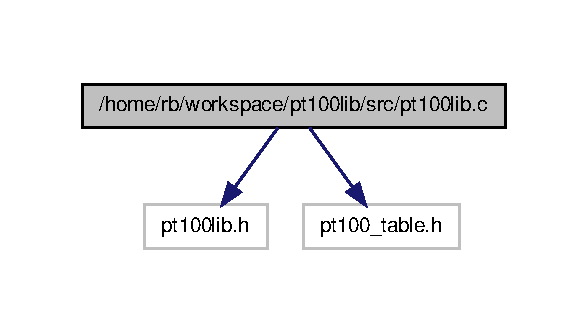
\includegraphics[width=282pt]{pt100lib_8c__incl}
\end{center}
\end{figure}
\subsection*{Funktionen}
\begin{DoxyCompactItemize}
\item 
\hyperlink{pt100__types_8h_ab4a3e130664d6751b5fd947f9b7382e0}{\_\-\_\-s32} \hyperlink{pt100lib_8c_a49de64016a5145d95be6830e2240d6bb}{pt100\_\-R2T} (\hyperlink{pt100__types_8h_a13a2835755bfba96b1790ff492741141}{\_\-\_\-u32} u32Widerstand)
\begin{DoxyCompactList}\small\item\em Wandelt einen PT100-\/Widerstandswert in eine Temperatur um. \item\end{DoxyCompactList}\item 
\hyperlink{pt100__types_8h_a13a2835755bfba96b1790ff492741141}{\_\-\_\-u32} \hyperlink{pt100lib_8c_a9346ef20f269515f671f6491077e5c70}{pt100\_\-T2R} (\hyperlink{pt100__types_8h_ab4a3e130664d6751b5fd947f9b7382e0}{\_\-\_\-s32} s32Temperatur)
\begin{DoxyCompactList}\small\item\em Wandelt eine Temperatur in einen Pt100 Widerstandswert. \item\end{DoxyCompactList}\end{DoxyCompactItemize}


\subsection{Ausführliche Beschreibung}
Bibiliothek mit PT100 Funktionen. \begin{DoxyAuthor}{Autor}
Roman Buchert (\href{mailto:roman.buchert@googlemail.com}{\tt roman.buchert@googlemail.com}) 
\end{DoxyAuthor}


Definiert in Datei \hyperlink{pt100lib_8c_source}{pt100lib.c}.



\subsection{Dokumentation der Funktionen}
\hypertarget{pt100lib_8c_a49de64016a5145d95be6830e2240d6bb}{
\index{pt100lib.c@{pt100lib.c}!pt100\_\-R2T@{pt100\_\-R2T}}
\index{pt100\_\-R2T@{pt100\_\-R2T}!pt100lib.c@{pt100lib.c}}
\subsubsection[{pt100\_\-R2T}]{\setlength{\rightskip}{0pt plus 5cm}{\bf \_\-\_\-s32} pt100\_\-R2T (
\begin{DoxyParamCaption}
\item[{{\bf \_\-\_\-u32}}]{u32Widerstand}
\end{DoxyParamCaption}
)}}
\label{pt100lib_8c_a49de64016a5145d95be6830e2240d6bb}


Wandelt einen PT100-\/Widerstandswert in eine Temperatur um. 


\begin{DoxyParams}{Parameter}
{\em u32Widerstand} & Widerstand in mOhm \\
\hline
\end{DoxyParams}
\begin{DoxyReturn}{Rückgabe}
Temperatur in °mC 
\end{DoxyReturn}


Temperatur berechnen \[ T = T1 + \frac{(T2-T1)*(R-R1)}{(R2-R1)} \] (T2 -\/T1) x (R -\/ R1) \par
 T = T1 + -\/-\/-\/-\/-\/-\/-\/-\/-\/-\/-\/-\/-\/-\/-\/-\/-\/-\/-\/ \par
 (R2 -\/ R1) \par


T : berechnete Temperatur \par
 T1 : Temperaturtabellenwert unter gemessenem Widerstand \par
 T2 : Temperaturtabellenwert über gemessenem Widerstand \par


R : gemessener Widerstand \par
 R1 : Widerstandstabellenwert unter gemessenem Widerstand \par
 R2 : Widerstandstabellenwert über gemessenem Widerstand \par


(Quelle: Elektrische Temperaturmessung (M. Nau / jumo))



Definiert in Zeile 23 der Datei pt100lib.c.



Benutzt INDEX\_\-MAX, INDEX\_\-ZERO, pt100\_\-table, R\_\-MAX, R\_\-MIN und T\_\-DIFF.

\hypertarget{pt100lib_8c_a9346ef20f269515f671f6491077e5c70}{
\index{pt100lib.c@{pt100lib.c}!pt100\_\-T2R@{pt100\_\-T2R}}
\index{pt100\_\-T2R@{pt100\_\-T2R}!pt100lib.c@{pt100lib.c}}
\subsubsection[{pt100\_\-T2R}]{\setlength{\rightskip}{0pt plus 5cm}{\bf \_\-\_\-u32} pt100\_\-T2R (
\begin{DoxyParamCaption}
\item[{{\bf \_\-\_\-s32}}]{s32Temperatur}
\end{DoxyParamCaption}
)}}
\label{pt100lib_8c_a9346ef20f269515f671f6491077e5c70}


Wandelt eine Temperatur in einen Pt100 Widerstandswert. 


\begin{DoxyParams}{Parameter}
{\em s32Temperatur} & Temperatur in m°C \\
\hline
\end{DoxyParams}
\begin{DoxyReturn}{Rückgabe}
Widerstand in mOhm 
\end{DoxyReturn}


Widerstand berechnen \[ R = R1 + \frac{(R2-R1)*(T-T1)}{(T2-T1)} \] (R2 -\/R1) x (T -\/ T1) \par
 R = R1 + -\/-\/-\/-\/-\/-\/-\/-\/-\/-\/-\/-\/-\/-\/-\/-\/-\/-\/-\/ \par
 (T2 -\/ T1) \par


T : berechnete Temperatur \par
 T1 : Temperaturtabellenwert unter gemessenem Widerstand \par
 T2 : Temperaturtabellenwert über gemessenem Widerstand \par


R : gemessener Widerstand \par
 R1 : Widerstandstabellenwert unter gemessenem Widerstand \par
 R2 : Widerstandstabellenwert über gemessenem Widerstand \par


(Quelle: Elektrische Temperaturmessung (M. Nau / jumo))



Definiert in Zeile 94 der Datei pt100lib.c.



Benutzt INDEX\_\-MAX, pt100\_\-table, T\_\-DIFF, T\_\-MAX und T\_\-MIN.


\hypertarget{pt100lib_8h}{
\section{/home/rb/workspace/pt100lib/includes/pt100lib.h-\/Dateireferenz}
\label{pt100lib_8h}\index{/home/rb/workspace/pt100lib/includes/pt100lib.h@{/home/rb/workspace/pt100lib/includes/pt100lib.h}}
}


Bibiliothek mit PT100 Funktionen.  


{\ttfamily \#include $<$pt100\_\-types.h$>$}\par
{\ttfamily \#include $<$stdlib.h$>$}\par
Include-\/Abhängigkeitsdiagramm für pt100lib.h:
\nopagebreak
\begin{figure}[H]
\begin{center}
\leavevmode
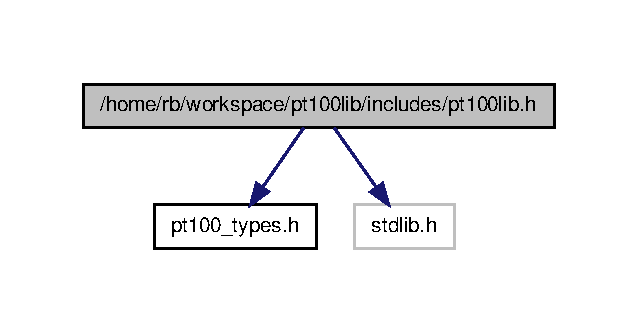
\includegraphics[width=306pt]{pt100lib_8h__incl}
\end{center}
\end{figure}
\subsection*{Funktionen}
\begin{DoxyCompactItemize}
\item 
\hyperlink{pt100__types_8h_ab4a3e130664d6751b5fd947f9b7382e0}{\_\-\_\-s32} \hyperlink{pt100lib_8h_a49de64016a5145d95be6830e2240d6bb}{pt100\_\-R2T} (\hyperlink{pt100__types_8h_a13a2835755bfba96b1790ff492741141}{\_\-\_\-u32} u32Widerstand)
\begin{DoxyCompactList}\small\item\em Wandelt einen PT100-\/Widerstandswert in eine Temperatur um. \item\end{DoxyCompactList}\item 
\hyperlink{pt100__types_8h_a13a2835755bfba96b1790ff492741141}{\_\-\_\-u32} \hyperlink{pt100lib_8h_a9346ef20f269515f671f6491077e5c70}{pt100\_\-T2R} (\hyperlink{pt100__types_8h_ab4a3e130664d6751b5fd947f9b7382e0}{\_\-\_\-s32} s32Temperatur)
\begin{DoxyCompactList}\small\item\em Wandelt eine Temperatur in einen Pt100 Widerstandswert. \item\end{DoxyCompactList}\end{DoxyCompactItemize}


\subsection{Ausführliche Beschreibung}
Bibiliothek mit PT100 Funktionen. \begin{DoxyAuthor}{Autor}
Roman Buchert (\href{mailto:roman.buchert@googlemail.com}{\tt roman.buchert@googlemail.com}) 
\end{DoxyAuthor}


Definiert in Datei \hyperlink{pt100lib_8h_source}{pt100lib.h}.



\subsection{Dokumentation der Funktionen}
\hypertarget{pt100lib_8h_a49de64016a5145d95be6830e2240d6bb}{
\index{pt100lib.h@{pt100lib.h}!pt100\_\-R2T@{pt100\_\-R2T}}
\index{pt100\_\-R2T@{pt100\_\-R2T}!pt100lib.h@{pt100lib.h}}
\subsubsection[{pt100\_\-R2T}]{\setlength{\rightskip}{0pt plus 5cm}{\bf \_\-\_\-s32} pt100\_\-R2T (
\begin{DoxyParamCaption}
\item[{{\bf \_\-\_\-u32}}]{u32Widerstand}
\end{DoxyParamCaption}
)}}
\label{pt100lib_8h_a49de64016a5145d95be6830e2240d6bb}


Wandelt einen PT100-\/Widerstandswert in eine Temperatur um. 


\begin{DoxyParams}{Parameter}
{\em u32Widerstand} & Widerstand in mOhm \\
\hline
\end{DoxyParams}
\begin{DoxyReturn}{Rückgabe}
Temperatur in °mC 
\end{DoxyReturn}


Temperatur berechnen \[ T = T1 + \frac{(T2-T1)*(R-R1)}{(R2-R1)} \] (T2 -\/T1) x (R -\/ R1) \par
 T = T1 + -\/-\/-\/-\/-\/-\/-\/-\/-\/-\/-\/-\/-\/-\/-\/-\/-\/-\/-\/ \par
 (R2 -\/ R1) \par


T : berechnete Temperatur \par
 T1 : Temperaturtabellenwert unter gemessenem Widerstand \par
 T2 : Temperaturtabellenwert über gemessenem Widerstand \par


R : gemessener Widerstand \par
 R1 : Widerstandstabellenwert unter gemessenem Widerstand \par
 R2 : Widerstandstabellenwert über gemessenem Widerstand \par


(Quelle: Elektrische Temperaturmessung (M. Nau / jumo))



Definiert in Zeile 23 der Datei pt100lib.c.



Benutzt INDEX\_\-MAX, INDEX\_\-ZERO, pt100\_\-table, R\_\-MAX, R\_\-MIN und T\_\-DIFF.

\hypertarget{pt100lib_8h_a9346ef20f269515f671f6491077e5c70}{
\index{pt100lib.h@{pt100lib.h}!pt100\_\-T2R@{pt100\_\-T2R}}
\index{pt100\_\-T2R@{pt100\_\-T2R}!pt100lib.h@{pt100lib.h}}
\subsubsection[{pt100\_\-T2R}]{\setlength{\rightskip}{0pt plus 5cm}{\bf \_\-\_\-u32} pt100\_\-T2R (
\begin{DoxyParamCaption}
\item[{{\bf \_\-\_\-s32}}]{s32Temperatur}
\end{DoxyParamCaption}
)}}
\label{pt100lib_8h_a9346ef20f269515f671f6491077e5c70}


Wandelt eine Temperatur in einen Pt100 Widerstandswert. 


\begin{DoxyParams}{Parameter}
{\em s32Temperatur} & Temperatur in m°C \\
\hline
\end{DoxyParams}
\begin{DoxyReturn}{Rückgabe}
Widerstand in mOhm 
\end{DoxyReturn}


Widerstand berechnen \[ R = R1 + \frac{(R2-R1)*(T-T1)}{(T2-T1)} \] (R2 -\/R1) x (T -\/ T1) \par
 R = R1 + -\/-\/-\/-\/-\/-\/-\/-\/-\/-\/-\/-\/-\/-\/-\/-\/-\/-\/-\/ \par
 (T2 -\/ T1) \par


T : berechnete Temperatur \par
 T1 : Temperaturtabellenwert unter gemessenem Widerstand \par
 T2 : Temperaturtabellenwert über gemessenem Widerstand \par


R : gemessener Widerstand \par
 R1 : Widerstandstabellenwert unter gemessenem Widerstand \par
 R2 : Widerstandstabellenwert über gemessenem Widerstand \par


(Quelle: Elektrische Temperaturmessung (M. Nau / jumo))



Definiert in Zeile 94 der Datei pt100lib.c.



Benutzt INDEX\_\-MAX, pt100\_\-table, T\_\-DIFF, T\_\-MAX und T\_\-MIN.


\printindex
\end{document}
